Every game has at least two states: playing and game over. \emph{Flat Hunt} has six states in total; three playing states and three game over states (see Figure x). These game states are defined in class \texttt{GAME\_CONSTANTS}:

\texttt{Agent\_stuck, Agent\_stuck, Agent\_caught, Agent\_escapes, Prepare\_state, Play\_state, Move\_state: INTEGER is unique}
\texttt{-- Possible states of the game.}
\begin{figure}[h]
  \centerline{\hbox{
    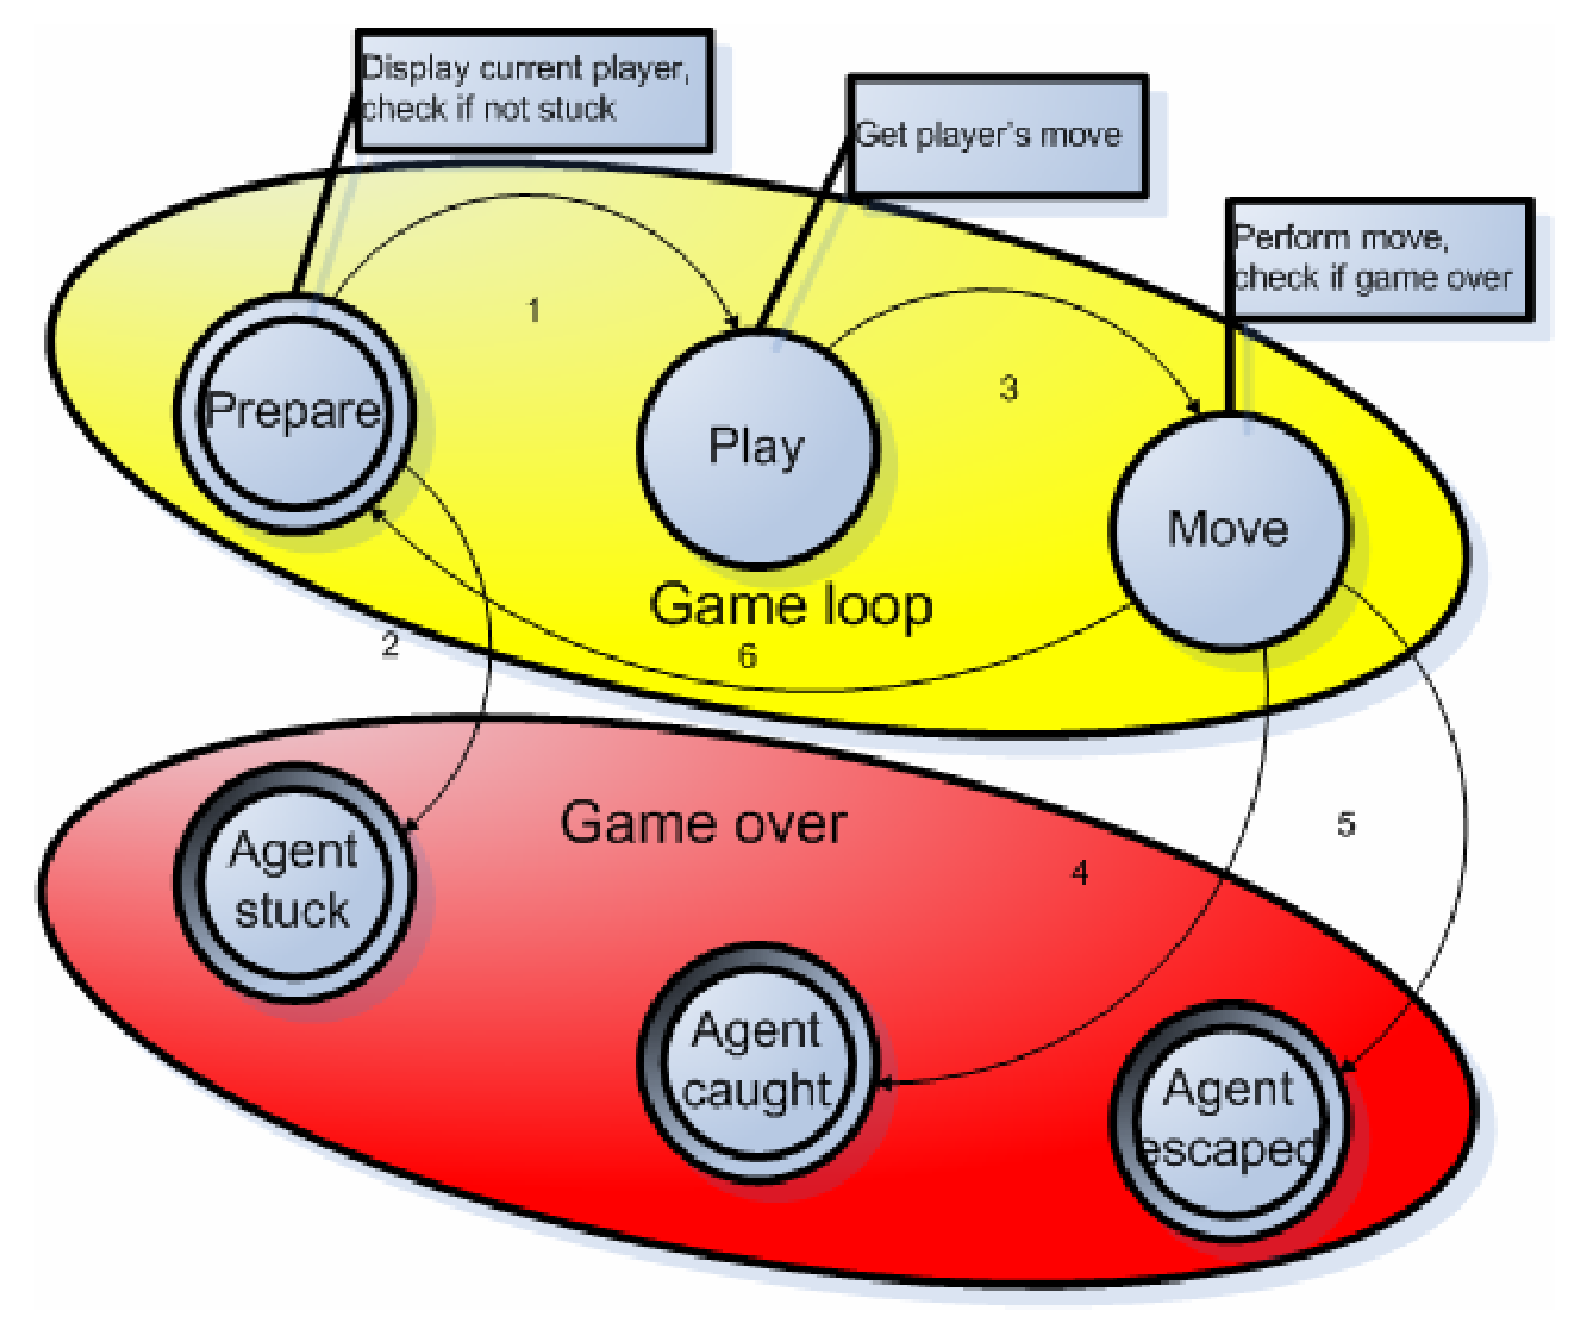
\includegraphics[width=120mm]{gameloop}
  }}
\caption{Game states and loop}
\label{gameloop}
\end{figure}
